\subsection{Pumpenansteuerung}
\label{subsec:Pumpenansteuerung}

Die 12 Pumpen werden direkt über den Mikrokontroller via Digitalausgänge angesteuert. Da jedoch der Mikrokontroller nicht genügend Strom liefern kann, wird ein Logik-MOSFET eingesetzt. Bei dem MOSFET handelt es scih um einen IRLR8726 von Infineon. Mit diesem wurde schon in früheren Projekten gearbeitet, bei welchen dieser zuverlässig arbeitete. Dieser MOSFET zeichnet sich durch einen geringen R$_{DSon}$ von 5.8m$\Omega$, eine kleine Gatekapazität von 15nC, einer V$_{DS}$ Breakdownvoltage von 30V und einer hohen Strombelastbarkeit von maximal 86A aus. Die Ansteuerung ist relativ simpel aufgebaut und kann in Abbildung \ref{fig:Pumpenansteuerung} begutachtet werden. 

\begin{figure}[h!]
\centering
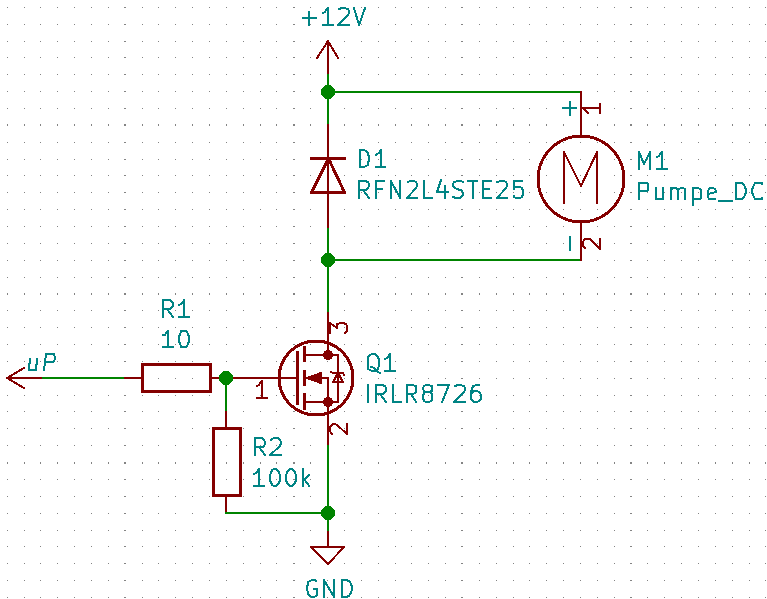
\includegraphics[width=0.6\textwidth]{graphics/Pumpenansteuerung.png}
\caption{Schema der Pumpenansteuerung}
\label{fig:Pumpenansteuerung}
\end{figure} 

Um den Gate-Eingang ein wenig zu schonen,wird ein 10$\Omega$ vogeschaltet. Parallel zum Motor ist eine Freilaufdiode verbaut, welche den Drain-Eingang der MOSFETS beim Ausschalten der Pumpe vor Spannungsspitzen schützt. 